\chapter{Évaluation}
\label{eval}

\section{Logiciels de construction}
\subsection{Java}
Pour tester les logiciels de construction nous avons compilé des projets de test de différent largeur sur les systèmes mesurant le temps.

\begin{table}[H]
\centering
\begin{tabular}{l|ccc} \toprule
	\textbf{Largeur} & \textbf{Ant (secondes)} & \textbf{Maven (secondes)} & \textbf{Gradle (secondes)}\\ \midrule
	Petit1 & 7.54 & 6.56 & 3.26\\
	Petit2 & 8.01 & 7.10 & 3.37\\
	Petit3 & 7.57 & 6.49 & 3.41\\
	Grand1 & 27.42 & 24.32 & 11.43\\
	Grand2 & 35.25 & 23.45 & 12.25\\
	Grand3 & 28.17 & 25.01 & 12.05\\ \bottomrule
\end{tabular}
\caption{Évaluation de logiciel de construction Java}
\end{table}
\subsubsection{Conclusion}
Gradle a des résultats meilleur que Ant et Maven, mais c'est plus compliqué a apprendre. Aussi la documentation de Gradle n'est pas très facile a comprendre parce-que elle est très détaillé.

\subsubsection{Comparaison de Syntaxe}
	\paragraph{Maven et Ant - pom.xml et build.xml}
		Tout les deux utilisent xml pour structurer les données. Le fichier pom.xml utilisé par Maven est court et net. Si on dit que Maven est comme une voiture, Ant est une collection des composants pour construire un véhicule. Il faut dire Ant exactement ce que il y a à faire. Pour cette raison le fichier build.xml deviens long et embrouillé très vite.
	\paragraph{Gradle - build.gradle}
		Gradle utilise un format basé sur JSON qui restes lisible aussi pour des projets grands. C'est possible d' ajouter des librairies dépendent construit avec Maven ou Ivy et de publier sur ces deux formes des répositoires.

\newpage
\section{Serveur de l'intégration continue}

\subsection{Définition des critères}

En dessous vous trouvez les critères avec une bref description qui seront utilisé pour évaluer les quatre serveurs de l'intégration continue qui ont été choisit pour ce travail. \footnote{\cite{ibmciserver}}

\begin{enumerate}
\item \textbf{Caractéristiques du produit} \\
\textit{Les caractéristiques du produit sont l'aspect le plus important quand on choisit un serveur d'IC. On doit savoir les exigences d'une entreprise et de ce point de vue sélectionner un logiciel.}
	\begin{itemize}
		\item Intégration avec des outils de gestion des versions \\
		\textit{Est l'outil que nous utilisons supporté? Quelles outils sont supporté?}
		\item Intégration avec l'outil de construction \\
		\textit{Est notre langage de programmation (compilateur) et notre outil de construction supporté?}
		\item Information en retour \\
		\textit{Quelles méthodes de l'information en retour existe et sont-ils suffisant pour nous?}
		\item Labeling \\
		\textit{Est-il possible de donner des identifiant à des versions d'un logiciel?}
		\item Extensibilité \\
		\textit{Est-il possible d'écrire des extension propre ou des plugins pour le serveur si nécessaire?}
	\end{itemize}
\item \textbf{Générale}
	\begin{itemize}
		\item Fiabilité et longévité
		\item Environnement cible
		\item Infrastructure
		\item Couts
		\item Type de logiciel
	\end{itemize}
\item \textbf{Taille de la communauté}
	\begin{itemize}
		\item Nombre d'utilisateurs
		\item Nombre de plugins
	\end{itemize}
\item \textbf{Utilisation}
	\begin{itemize}
		\item Facilité d'utilisation
		\item Complexité de l'installation
	\end{itemize}
\end{enumerate}
\newpage
\begin{landscape}
\begin{table}[H]
	\centering
		\begin{tabular}{lp{4cm}p{4cm}p{4cm}p{4cm}} \toprule
			\textbf{Critères} & \href{https://jenkins-ci.org}{\textbf{Jenkins}} & \href{https://www.jetbrains.com/teamcity/}{\textbf{TeamCity}} & \href{https://travis-ci.org}{\textbf{Travis CI}} & \href{https://www.visualstudio.com/en-us/products/tfs-overview-vs.aspx}{\textbf{Team Foundation Server}} \\ \midrule
			\rowcolor{GrayRow}\textbf{Caractéristique du produit} &  &  &  &  \\ \midrule[0.16em]
			Outils de gestion des versions & Subversion/CVS(+plugins) & Subversion/CVS(+plugins) & github/Git & Git/TFVC \\ \midrule
			Outils de construction &  \checkmark & \checkmark\checkmark (CLI) & \checkmark & \checkmark \\ \midrule
			Information en retour & \checkmark (Courriel, Plugins) & \checkmark & \checkmark\checkmark & \checkmark\checkmark \\ \midrule
			Labeling &  \checkmark\checkmark & \checkmark & - - &\checkmark\checkmark \\ \midrule
			Extensibilité & \checkmark\checkmark & \checkmark & - & \checkmark \\ \midrule
			\rowcolor{GrayRow}\textbf{Générale} &  &  &  &  \\ \midrule[0.16em]
			Fiabilité et longévité & \checkmark\checkmark & \checkmark\checkmark & \checkmark\checkmark & \checkmark\checkmark \\ \midrule
			Environnement cible & multi-plateforme & multi-plateforme & Linux & Microsoft Windows \\ \midrule
			Infrastructure & On-premises & On-premises & On-premises/SaaS & On-premises/SaaS \\ \midrule
			Couts & gratuit & Freemium* & Freemium* & Freemium \\ \midrule
			Type de logiciel & Open Source (MIT) & Propriétaire & Open Source (MIT) & Propriétaire \\ \midrule
			\rowcolor{GrayRow}\textbf{Taille de la communauté} & & & & \\ \midrule[0.16em]
			Nombre d'utilisateurs & 127'000 & 30'000 clients & 240'000 projets & Many \\ \midrule
			Nombre de plugins & \checkmark\checkmark & \checkmark & - - & - \\ \midrule
			\rowcolor{GrayRow}\textbf{Utilisation} &  &  &  &  \\ \midrule[0.16em]
			Facilité d'utilisation & \checkmark & \checkmark & \checkmark\checkmark & \checkmark\checkmark \\ \midrule
			Complexité de l'installation & \checkmark & \checkmark & \checkmark\checkmark &  \checkmark\checkmark\\
			\bottomrule[0.16em]
		\end{tabular}
	\caption{Serveurs de l'IC}
	\label{tab:serveurs_eval}
\end{table}
\checkmark\checkmark = très bien | \checkmark = bien | - = déficient | - - = pas existant/suffisant \\
Freemium = C'est gratuit pour la version base, mais ça coute pour des éditions plus grande (entreprise).\\
On-premises = Les serveurs pour y installer le logiciel sont fourni par le client.\\
SaaS = Software as a Service \\
* gratuit pour des projets Open Source
\footnote{\citep{jenkinsplugins} \citep{teamcityenv} \citep{tfsversioncontrol}}


\end{landscape}
\newpage

\subsection{Jenkins}
\begin{wrapfigure}{r}{0.2\textwidth}
  \begin{center}
    
\includegraphics[width=0.18\textwidth]{bilder/JENKINS}
  \end{center}
  \caption{Jenkins Logo}
\end{wrapfigure}
\paragraph{Caractéristique du produit} Bien que Jenkins est écrit en Java il est capable de construire beaucoup des langues différents, comme PHP, Ruby, .Net avec des plugins. Tout les autres langage peuvent lancer un script batch ou shellscript dépendent au système d'exploitation. Il y a une nouvelle version de Jenkins chaque semaine (utilisant IC avec soi-même trouvé sur https://www.jenkins-ci.org/).

\paragraph{Générale} Jenkins est un fork de l'outil Hudson qui était développe par Kohsuke Kawaguchi chez Sun Microsystems en 2008. Deux ans plus tard Kohsuke a eu des différences avec son nouveau employeur Oracle. Il a quitté et en 2011 présente la première version de Jenkins. Jenkins est un logiciel code source ouvert écrit en Java licenciée MIT. 
\paragraph{Taille de la communauté} Aujourd'hui Jenkins est installé sur 127'000 machines\footnote{\citep{jenkinsstats}}. Sur la site web officielle de Jenkins il y a des plugins à toutes fins.(1000++) 
\paragraph{Utilisation} Après lancer le service de Jenkins on peut ouvrir l'interface web sur 127.0.0.1:8080. Là on peut définir des jobs de construction, gérer les droits d'accès, changer des paramètres et beaucoup plus. Au début le système gestion de version Git n'était pas inclue, seulement CVS et SVN mais aujourd'hui il y a un plugin. L'interface d'administration est très facile à utiliser.
\begin{figure}[H]
	\centering
		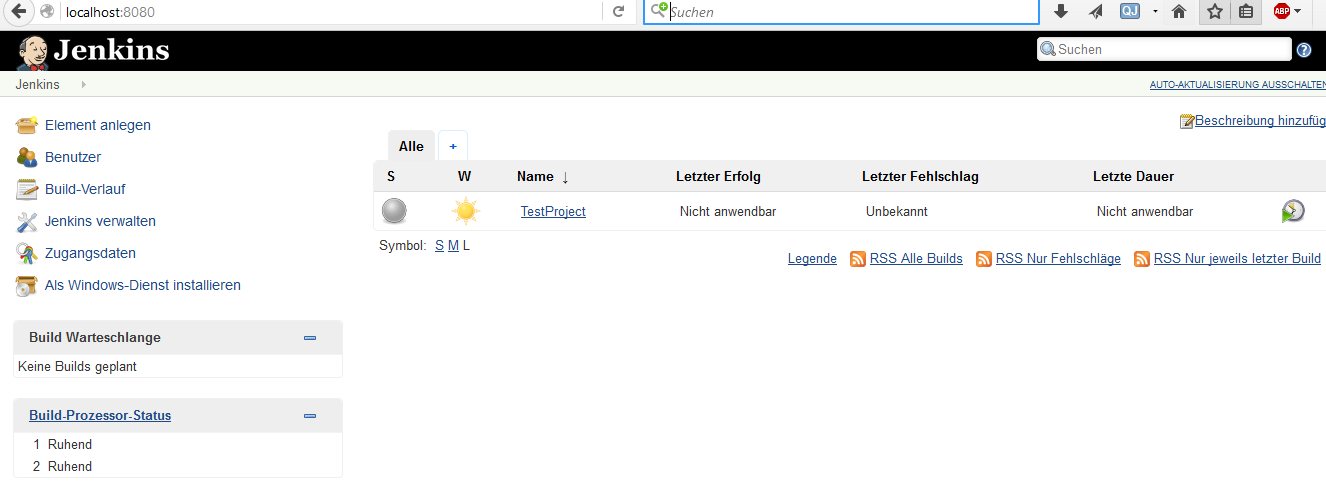
\includegraphics[width=15cm]{bilder/JenkinsGui}
	\caption{Jenkins intérface d'administration}
	\label{fig:jenkinsgui}
\end{figure}

\clearpage


\subsection{TeamCity}
\begin{wrapfigure}{r}{0.2\textwidth}
  \begin{center}
    
\includegraphics[width=0.18\textwidth]{bilder/teamcity512}
  \end{center}
  \caption{TeamCity Logo}
\end{wrapfigure}
\paragraph{Caractéristique du produit} TeamCity est un serveur de l'intégration continue de JetBrains, les fabricants d'une grande nombre d'outil de développement (comme IntelliJ). Il est optimisé pour construire des projets de Java ou .NET, mais supporte aussi Python, Ruby et beaucoup d'autre langage avec des plugins. De plus il existe l'option de travailler avec la ligne de commande. TeamCity est très adaptable et peut être individualiser extensivement. \\
Tous les configurations et tous l'utilisation est effectué par l'interface web. Comme voies d'information en retour TeamCity supporte des emails, des messages Jabber ou des notifications directement dans l'IDE. De plus TeamCity supporte des "Build Tag" pour identifier des constructions. Si la fonctionnalité de TeamCity ne suffit pas, il est facilement possible d'écrire un plugin.

\paragraph{Générale} L'infrastructure pour soutenir TeamCity doit être mis en place par l'entreprise. Il existe trois options de licence de TeamCity.
\begin{itemize}
	\item TeamCity Professional (20 configurations et 3 agent de construction)
	\item TeamCity Enterprise (3-100 agent packs)
	\item TeamCity Additional Build Agent (+ 1 agent de construction)
\end{itemize}
La licence TeamCity Professional est gratuite mais limité. Pour les versions TeamCity Enterprise le nombre de projets est illimité mais payant (commençant de xxx) , mais on peu incrémenter le nombre d'agent de construction pour atteindre une meilleure performance quand il y a beaucoup de processus de construction parallèle. Pour des projets Open Source TeamCity est gratuite, pour des jeunes pousses il y a des rabais.\footnote{\citep{teamcitybuy}}
\paragraph{Taille de la communauté}
JetBrains affirme que 30'000+ clients utilise TeamCity pour exécuter l'intégration continue (Boeing, HP...). Il y a une grande nombre de plugins disponible sur le page web de TeamCity.\footnote{\citep{teamcityplugins}}
\paragraph{Utilisation}
L'installation de TeamCity est assez facile. Il existe des archive des fichiers exprès pour des installations rapide. TeamCity est basé sur Java et utilise un serveur Tomcat. Pour l'installation rapide, tous ce qu'on doit faire est télécharger et extraire l'archive, et puis exécuter un script et compléter la configuration initiale. Pour un système productive une installation un peu plus complexe est prévu.\\
En utilisant TeamCity en premier on est confondu par la grande nombre d'options de configuration. Mais quand-même il était possible et pas très difficile de construire et mettre en rapport notre environnement teste. TeamCity est très volumineux, mais bien structuré et agréable pour l'utilisateur. Le faite qu'on peut faire toute la configuration sur l'interface web est un grande plus.
\begin{figure}[H]
	\centering
		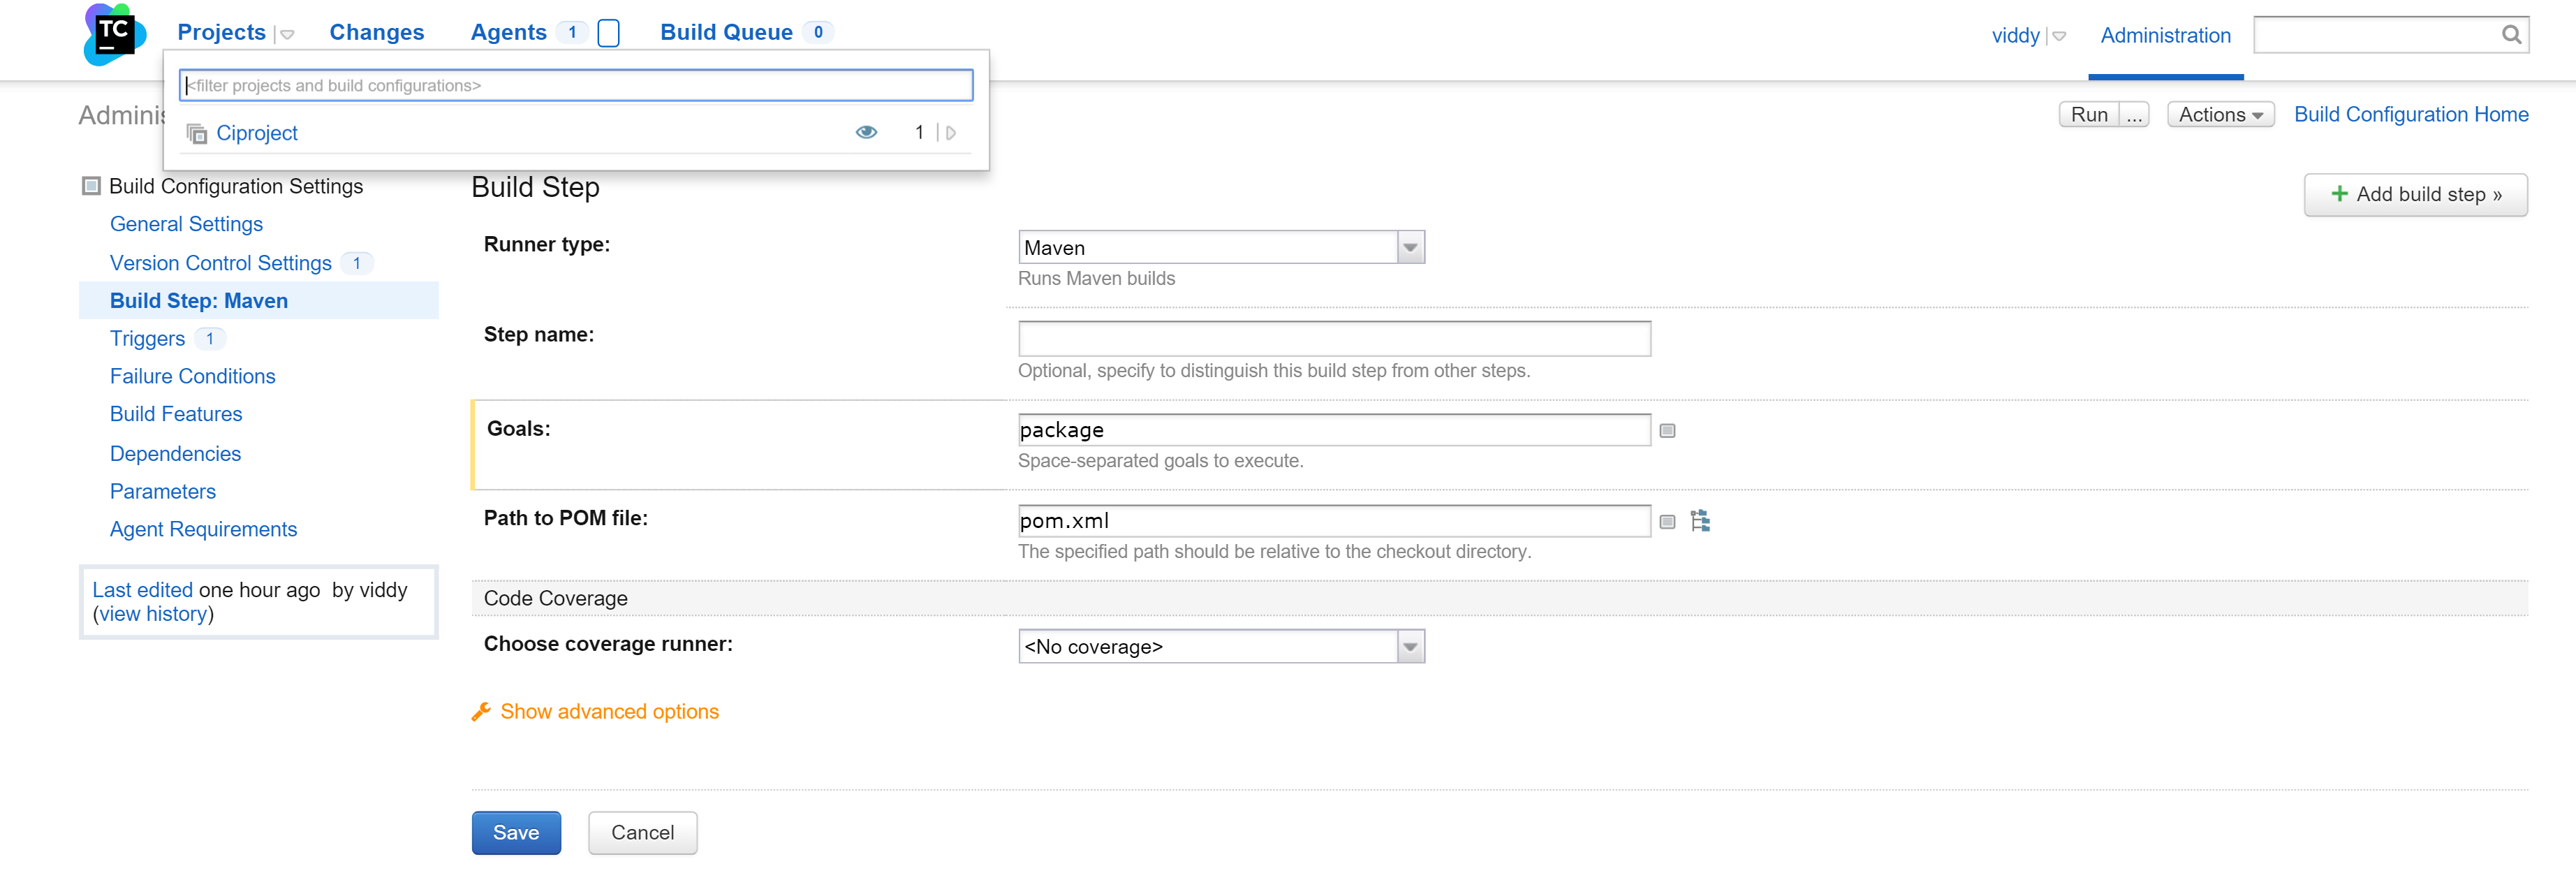
\includegraphics[scale=0.35]{bilder/teamcityadmin}
	\caption{TeamCity interface d'administration}
	\label{fig:travisgui}
\end{figure}





\clearpage
\subsection{Travis CI}
\begin{wrapfigure}{r}{0.4\textwidth}
  \begin{center}
    
\includegraphics[width=0.38\textwidth]{bilder/Travis-CI-logo}
  \end{center}
  \caption{Travis CI Logo}
\end{wrapfigure}
\paragraph{Caractéristique du produit}
Travis CI est un serveur de l'intégration continue très facile à mettre en service et avec une intégration excellente avec \href{https://github.com/}{github.com}. Il supporte beaucoup de différent langage et outil de construction. La liste complète peuvent être trouver dans la documentation\footnote{\citep{traviscidocs}}. Travis seulement supporte git comme outil de gestion des versions.\\
De plus il offre multiple voies d'information en retour. Le plus facile est par email, mais il y a aussi la possibilité d'envoyer des messages par IRC, Slack, HipChat etc.\footnote{\citep{traviscinotification}}. Chaque construction reçoit un identificateur numérique, mais il n'est pas possible de le changer. Il y a une API pour accéder à Travis (SaaS), mais l'extensibilité semble limité.

\paragraph{Générale}
Il existe trois version de Travis CI.
\begin{itemize}
	\item \href{https://travis-ci.org/}{Travis CI for Open Source}
	\item \href{https://travis-ci.com/}{Travis Pro}
	\item \href{https://enterprise.travis-ci.com/}{Travis Enterprise}
\end{itemize}
Les deux première versions sont accessible comme SaaS. Une version est pour des projets Open Source qui est gratuite et l'autre est pour des projets avec un dépôt de github privée qui est payant. La troisième version est pour des entreprises qui veulent mettre l'infrastructure à disposition eux-mêmes (Linux).

\paragraph{Taille de la communauté}
Travis CI affirme sur la page web qu'il y a 246'506 projets Open Source qui sont testé et intégré sur leur plateforme. Sur la nombre d'utilisateurs des deux versions commercial il n'y a pas d'information.

\paragraph{Utilisation}
L'utilisation de Travis CI est très pratiques est facile. Si on a déjà un dépôt sur github, il faut seulement trois pas pour lancer l'intégration continue avec Travis.

\begin{enumerate}
	\item Login avec le compte de github sur travis
	\item Choisir le dépôt
	\item Écrire un fichier .travis.yml pour définir la configuration
\end{enumerate}

Après ça chaque fois qu'il y a un changement sur le dépôt les tests et la construction seras exécuté automatiquement. Pour construire notre projet de test en java (maven), d'exécuter les testes avec trois différent version de java et envoyer un email à une adresse si quelque chose ne marche pas, le fichier en bas suffisait. De plus vous trouver un aperçu de l'interface d'administration de Travis.

\begin{figure}[H]
	\centering
		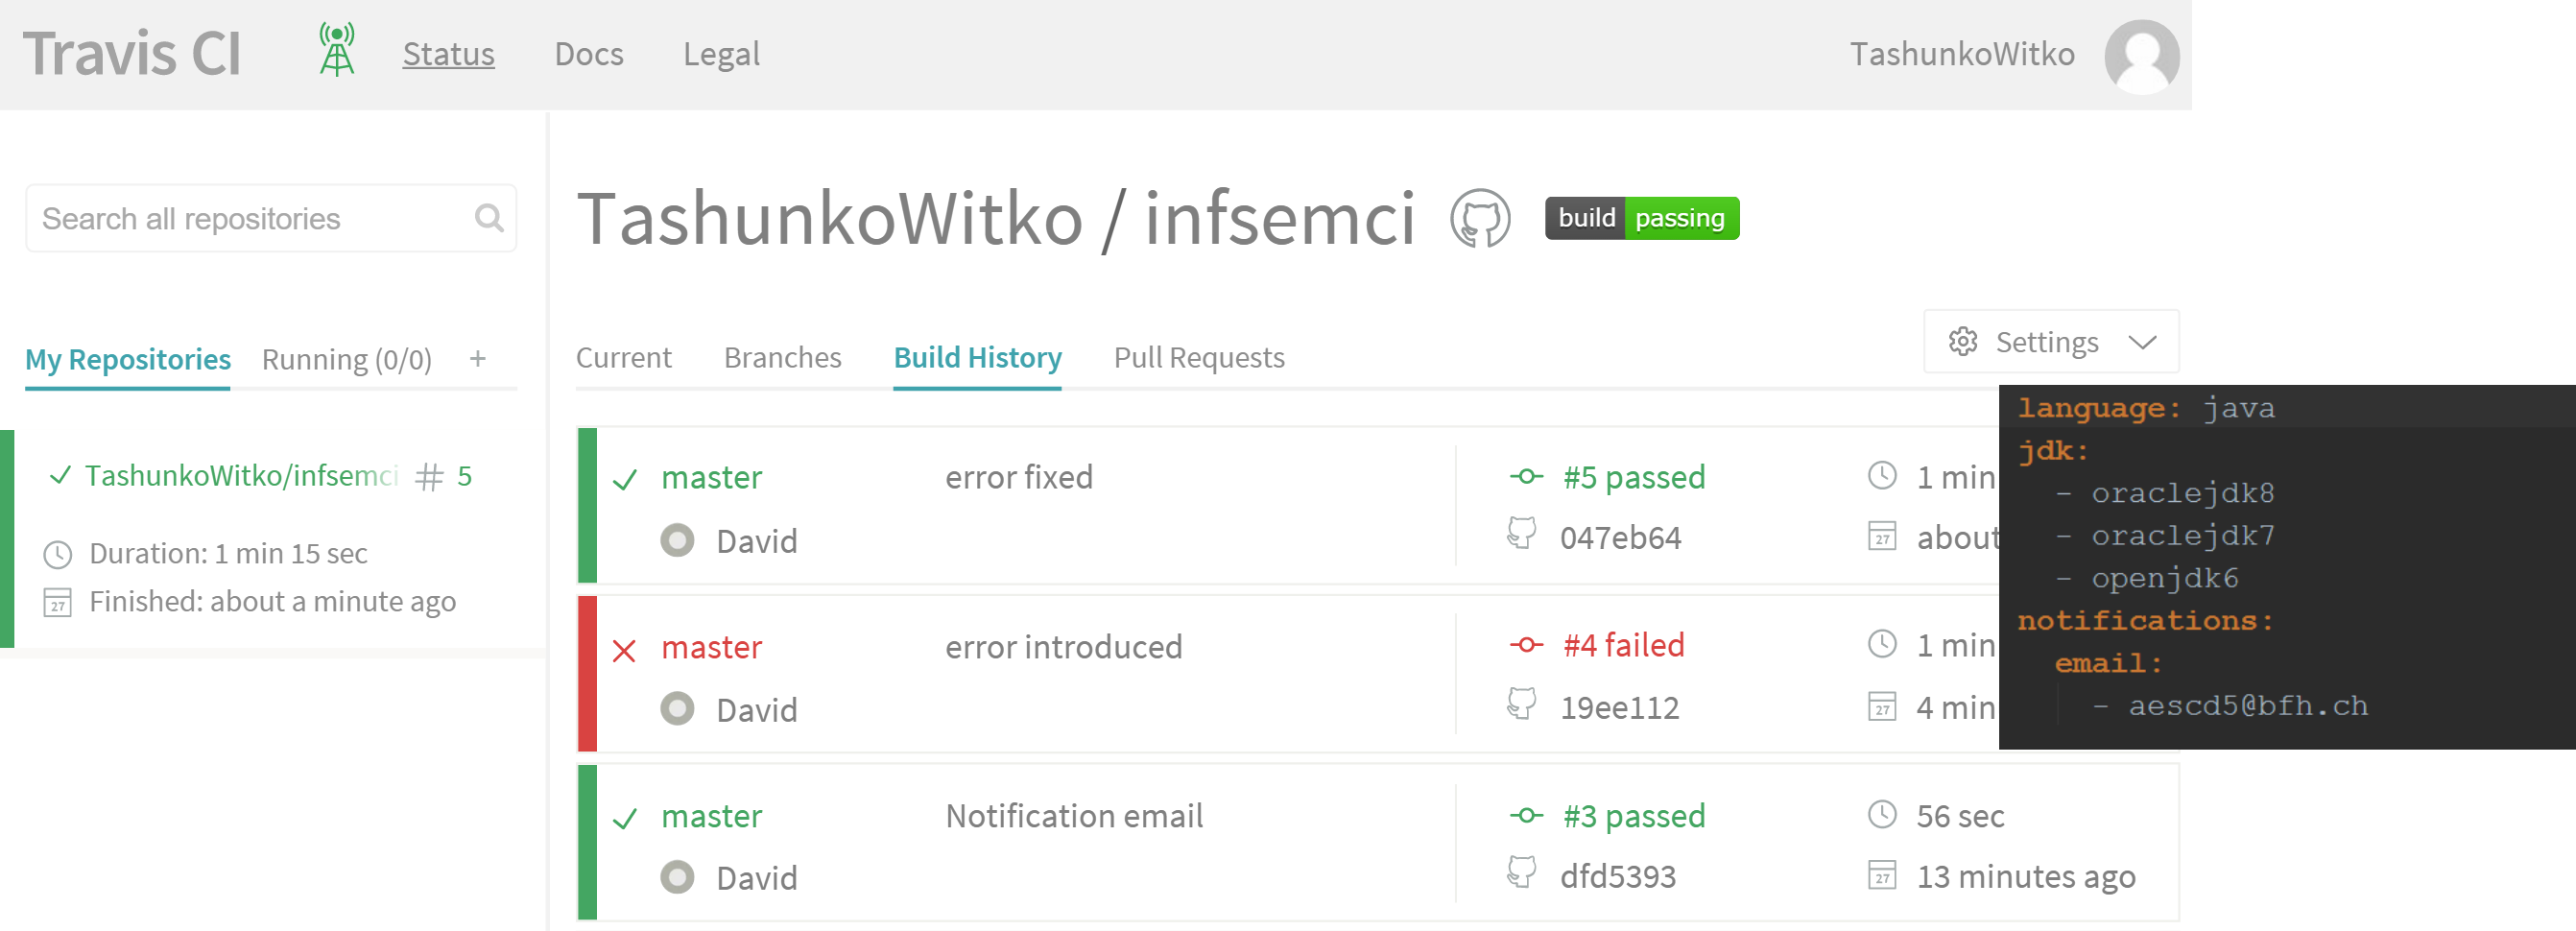
\includegraphics[scale=0.2]{bilder/travisciymlfile}
	\caption{Travis intérface d'administration et yml fichier}
	\label{fig:travisgui}
\end{figure}
\clearpage



\subsection{Team Foundation Server}
\paragraph{Caractéristique du produit} TFS est de la forge logicielle de Microsoft. Le cycle de vie entier du développement logiciel agile est couvert. La gestion des versions (TFVC ou Git), des constructions, des résultats de test et beaucoup plus car on peut installer des plugins gratuit et payée facilement. Il y a une version "On-premises" qui est installé sur une machine/un serveur de l'entreprise mise a jour une foi par trimestre par Windows Update Services. Si on veut avoir la version la plus actuelle à n'importe quel temps il y a un service en ligne, fourni par Microsoft sur la nuage Azure.

\paragraph{Générale}  Le prix pour la version "On-premises" est calculé également pour la version SaaS listé en bas.
\begin{table} [H]
	\centering
		\begin{tabular}{l|c} \toprule
			\textbf{Taille} & \textbf{Couts} \\ \midrule
			<5 personnes & Gratuit, Temps de construction inclue 240 minutes/mois \\
			6-10 personnes & CHF 5.40/personne et mois \\
			11-100 personnes & CHF 7.20/personne et mois\\
			101-1000 personnes & CHF 3.60/personne et mois \\
			>1001 personnes & CHF 1.80/personne et mois \\ \midrule
			Agent de construction additionnel (hosted) & CHF 36.10/agent \\
			Agent de construction additionnel (locale) & CHF 13.50/agent \\ \bottomrule
		\end{tabular}
	\caption{TFS Couts}
\end{table}
Combiné avec une suscription MSDN beaucoup des services VisualStudio et Azure sont inclue.
\paragraph{Taille de la communauté} Sur le nouveau magasin en ligne on peut télécharger nombreux plugins publié par Microsoft ou des développeurs indépendantes. Il y a des addons pour Visual Studio, VisualStudioCode et VisualStudio TeamServices gratuit et payé.
\paragraph{Utilisation} L'interface utilisateur est très intuitive. Après l'enregistrement on peut lier un projet locale avec le projet team en ligne. Si on veut configurer la construction ou le déploiement automatisé il faut ouvrir l'interface web et suivre les instructions. 
La partie test est un peu confus au début, parce que les tests unitaires et les tests d'intégration sont inclue dans la construction et dans le chapitre test sont les tests d'acceptation recordé.

\begin{figure}[H]
	\centering
		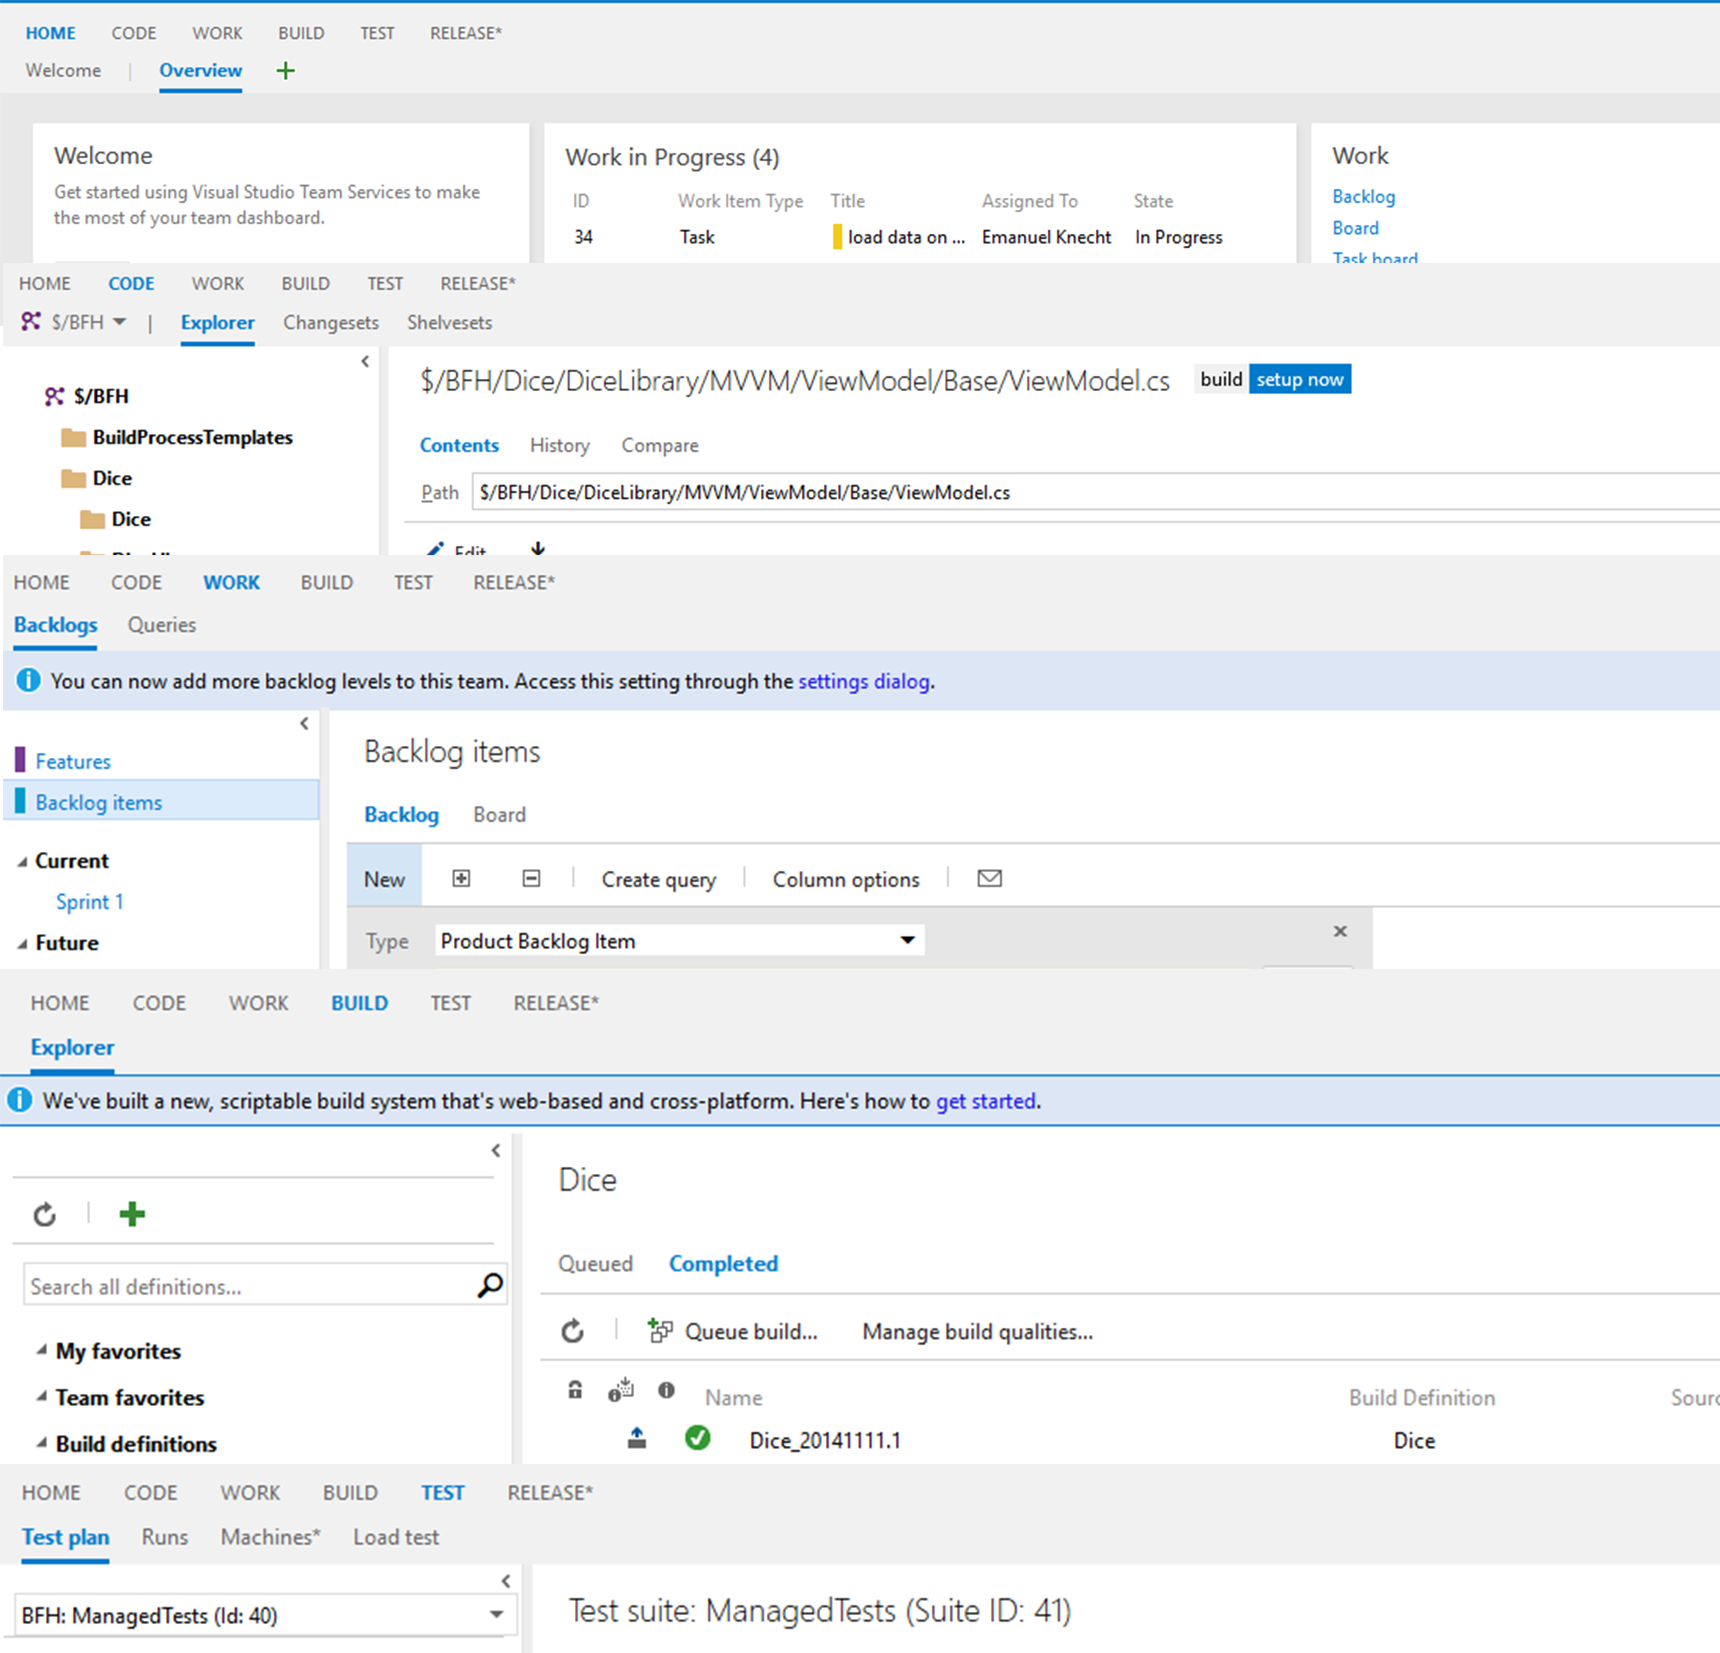
\includegraphics[height=8cm]{bilder/vso}
	\caption{Visualstudio Online interface d'administration}
	\label{fig:vsogui}
\end{figure}

